Consider the used-car data in Exercise 4.26.
\begin{enumerate}[label= (\alph*)]
    \item Determine the power transformation $\hat{\lambda}_{1}$ that makes the $x_{1}$ values approximately normal. Construct a Q-Q plot for the transformed data.
    
    \begin{figure}[H]
        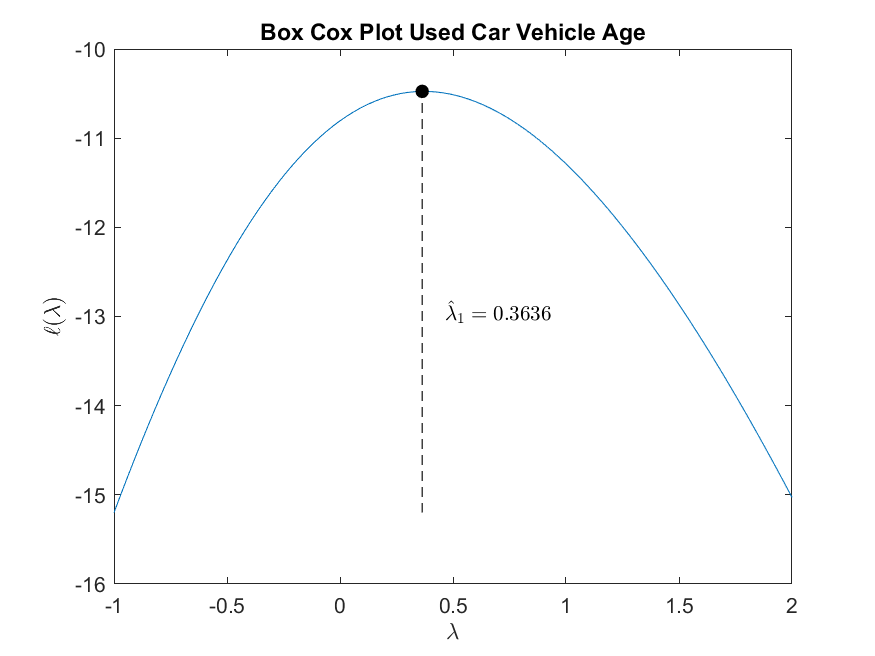
\includegraphics[scale=0.8]{./matlab/chapter-4/sol4.30a.png}
    \end{figure}

    \item Determine the power transformation $\hat{\lambda}_{2}$ that makes the $x_{2}$ values approximately normal. Construct a Q-Q plot for the transformed data.
    
    \begin{figure}[H]
        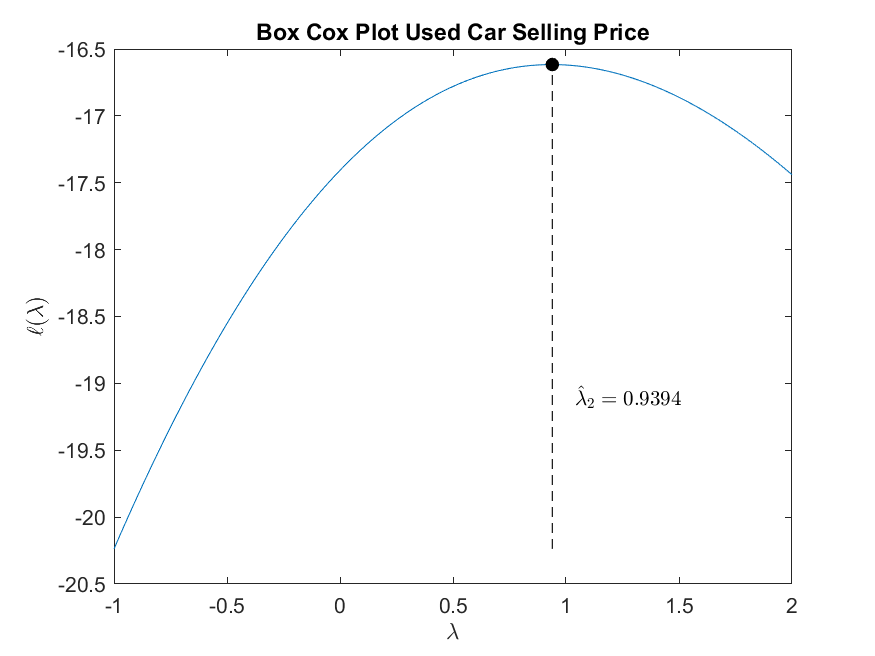
\includegraphics[scale=0.8]{./matlab/chapter-4/sol4.30b.png}
    \end{figure}

    \item Determine the power transformations $\hat{\bm{\lambda}}^{\prime} = [\hat{\lambda}_{1}, \hat{\lambda}_{2}]$ that make the $[x_{1}, x_{2}]$ values
    jointly normal using (4--40). Compare the results with those obtained in Parts a and b.
    
    \begin{figure}[H]
        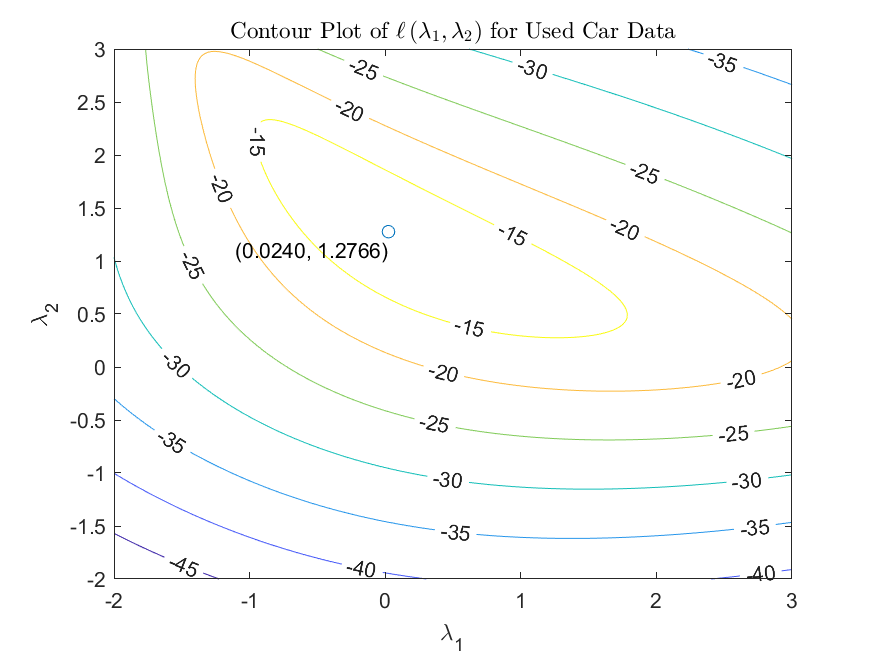
\includegraphics[scale=0.8]{./matlab/chapter-4/sol4.30c.png}
    \end{figure}
    \begin{figure}[H]
        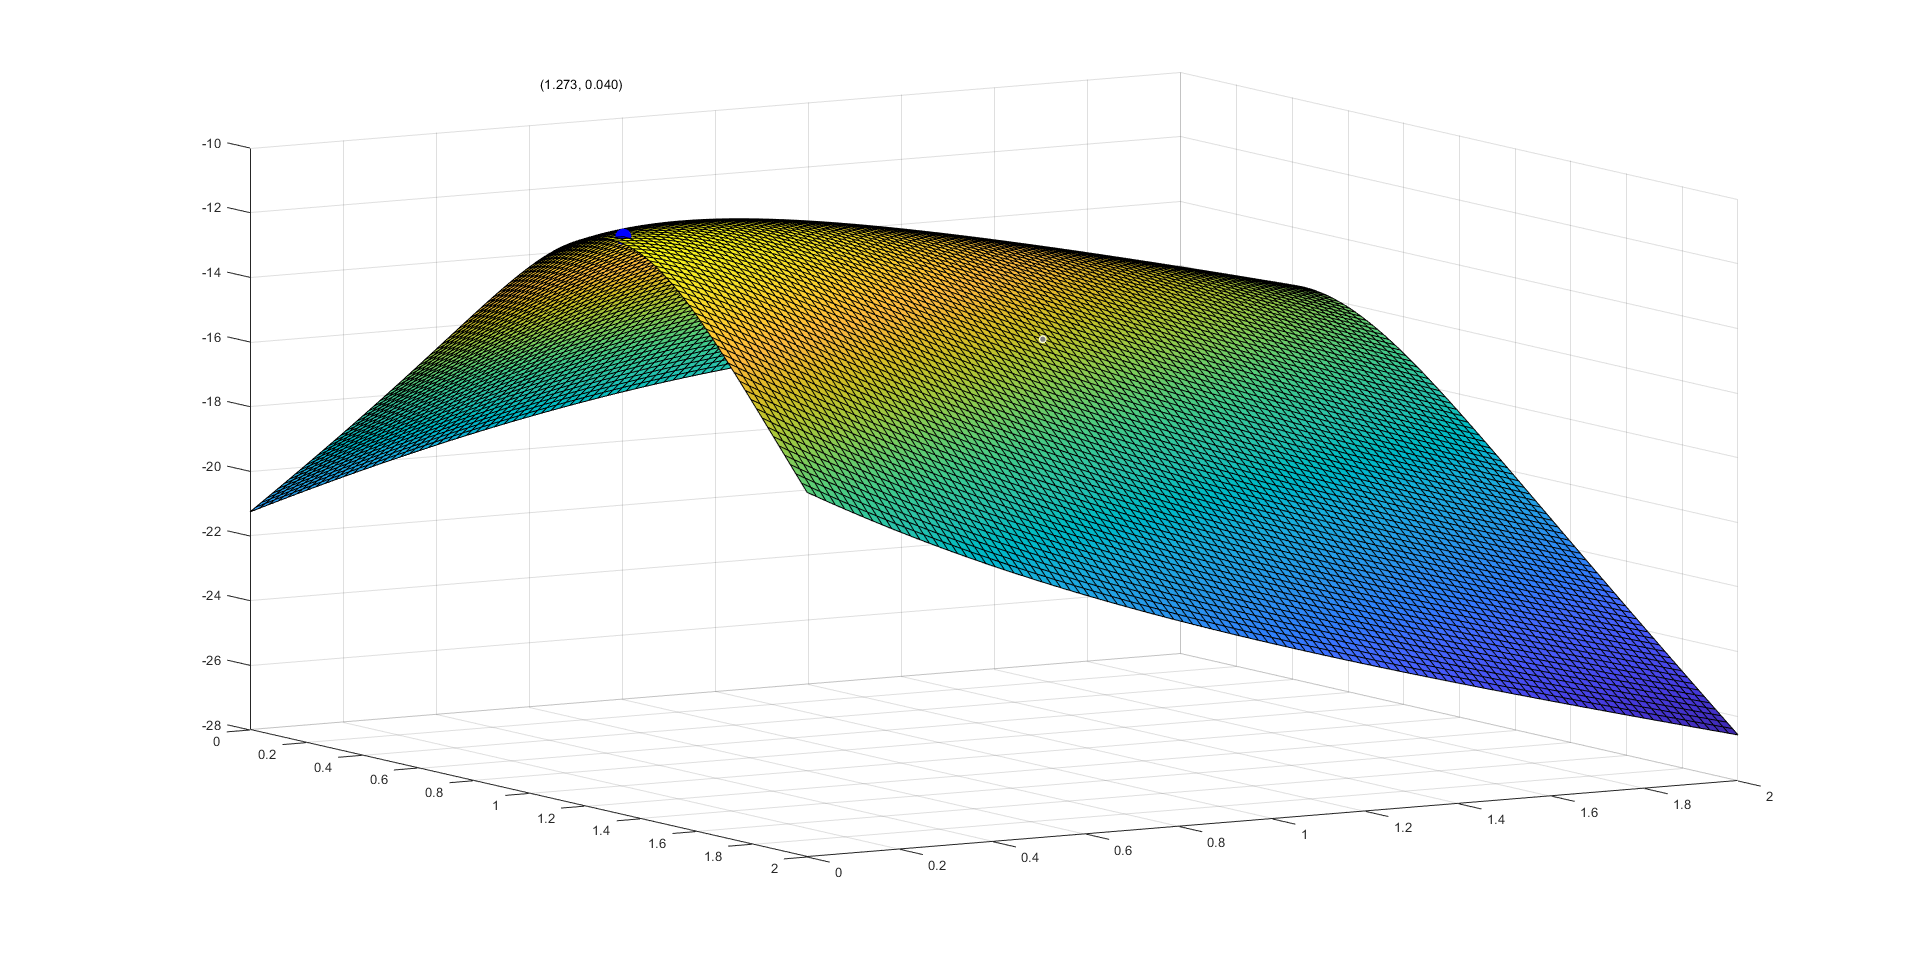
\includegraphics[scale=0.8]{./matlab/chapter-4/sol4.30c_surf.png}
    \end{figure}
    \par
    Using the joint distribution of $x_{1}$ and $x_{2}$,
     the simultaneous maximum for the \"best\" power transformation
     was found at $\hat{\bm{\lambda}}^{\prime} = [\hat{\lambda}_{1}, \hat{\lambda}_{2}] = [0.0202, 1.2828]$.
    That is, for vehicle age was $\hat{\lambda}_{1} = 0.0202$, and for sale price was $\hat{\lambda}_{2} = 1.2828$.
    These are a bit different from parts a and b where we were maximizing the univariate likelihood.
    In those cases the maximum for vehicle age was $\hat{\lambda}_{1} = 0.3636$ and for vehicle price was $\hat{\lambda}_{2} = 0.9394$.
\end{enumerate}